\begin{figure}
    \begin{center}
    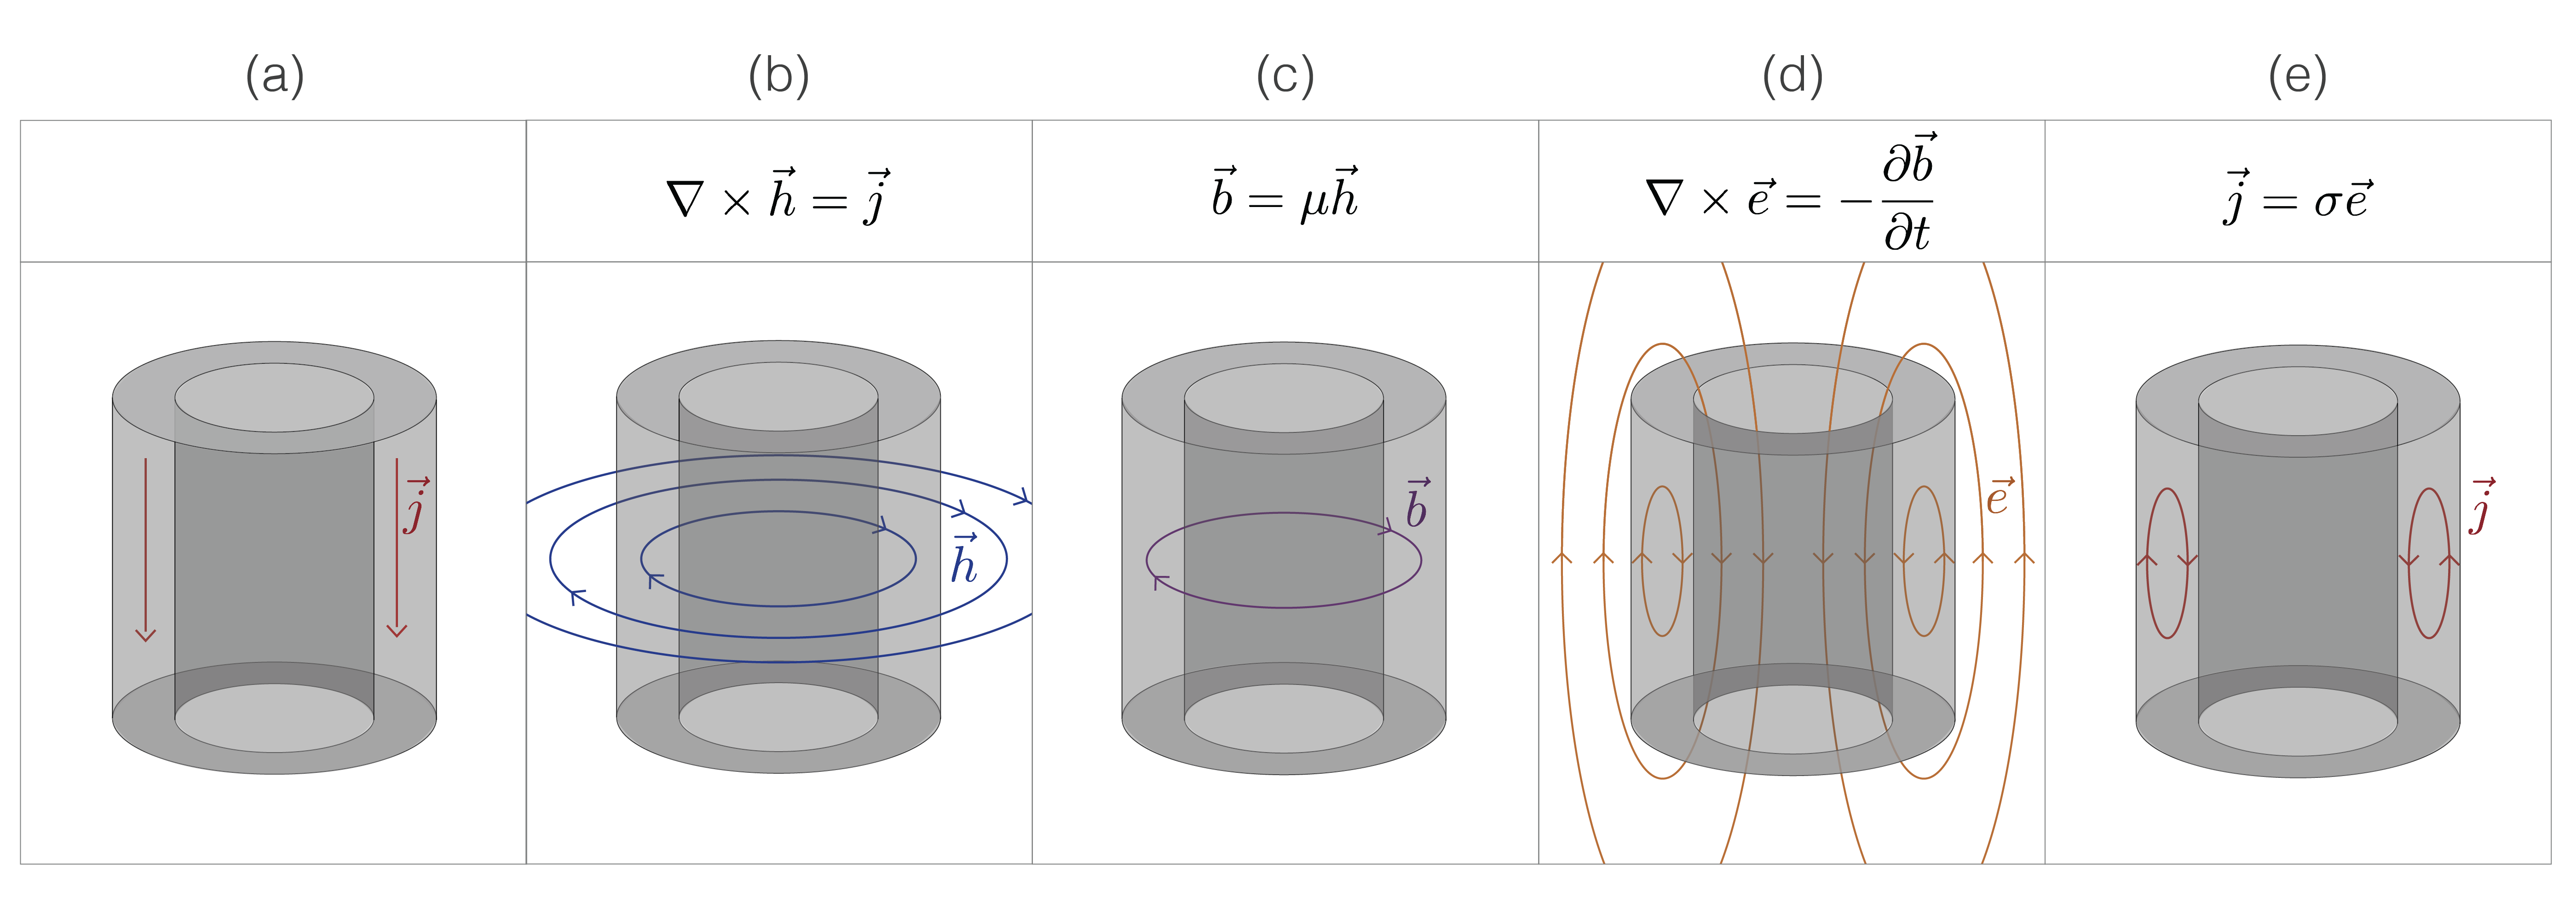
\includegraphics[width=\textwidth]{figures/casing-mu-sketch.png}
    \end{center}
\caption{
    Sketch demonstrating how a poloidal current system can arise inside of a conductive, permeable casing.
    A source current is applied and (a) currents flow downwards through the pipe. (b) Currents generate rotational magnetic fields according
    to Ampere's law. (c) Magnetic flux density is concentrated in the permeable pipe according to the constitutive relation between $\vec{b}$ and $\vec{h}$.
    (d) The magnetic flux varies with time creating rotational electric fields according to Faraday's law.
    (e) Currents associated with those electric fields are concentrated in conductive regions of the model in accordance with Ohm's law.
}
\label{fig:casing-mu-sketch}
\end{figure}



